\section{An overview of reduction methods}

The torque ripple minimization has been studied extensively for many years and numerous solutions have been already proposed. This chapter discusses the limitations and strengths of the already existing solutions. The focus is on software methods, although the machine design based methods are briefly outlined to provide an extensive overview. The software methods can be divided into three categories: algorithms that exploit foreknowledge, observer based methods and iterative methods. Fig. \ref{minimization_methods} summarizes the various torque ripple minimization methods presented in this chapter.
\textbf{\textbf{}}\begin{figure}[ht] 
    \centering
    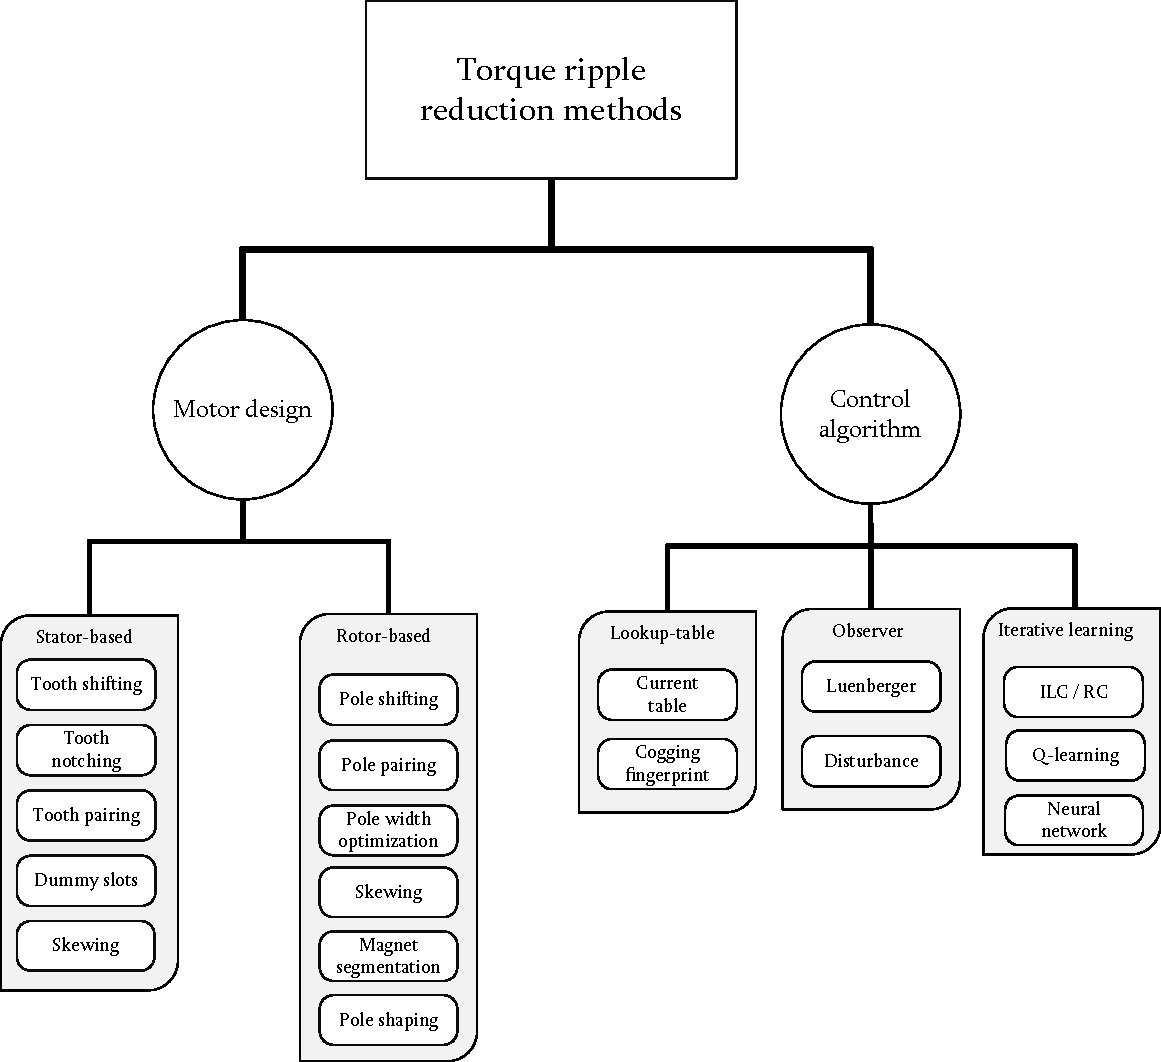
\includegraphics[width=1\linewidth]{images/minimization_methods.pdf} 
    \caption{Various torque pulsation reduction techniques}
    \label{minimization_methods} 
\end{figure}


\subsection{Machine design optimization}

Torque pulsation due to cogging torque emerge even if the machine is not excited by external voltage source. Therefore, it is logical to try reduce torque pulsations by addressing the sources and then improving the machine geometry appropriately. Design optimization has been found an effective way to reduce ripples. This explains the great number of different methods that can be further categorized to stator and rotor based methods \cite{CTR_HW:2013}. Rotor geometry optimization is often preferred over stator geometry optimization, because the rotor structure is simpler and thus easier to modify in PM machines \cite{TRR:1999, CTR_HW:2013}.

Cogging torque should be minimized in order to reduce torque ripple. Minimization techniques include for example, stator and rotor skewing \cite{CTR_HW:1994, CTR_HW:2001, CTR_HW:2002, CTR_Analytical:2009, CTR_HW:2013}, magnet arc width optimization \cite{CTR_HW:2002, CTR_HW:2003, CTR_HW:2001}, magnet pole shaping \cite{CTR_HW:1994, CTR_HW:2004}, magnet segmentation \cite{CTR_HW:2002, CTR:2010, CTR_SW:2017}, stator tooth notching \cite{CTR_HW:1994, CTR_HW:2002}, using odd number of slots \cite{CTR_HW_SLOTN:2011} and pole and teeth pairing \cite{CTR_HW:2001}. All these methods aim to improve the geometry of the machine that leads to reduced cogging torque. However, optimization is often a trade-off with other properties of the machine. Therefore, applying all the design improvements simultaneously is not necessarily practical or even possible \cite{CTR_HW:2002, CTR_HW:2013}.

Although, the geometry optimization is an effective way to reduce torque ripple, it is rarely an applicable solution when the machine has been manufactured already. Individual parts or the entire machine would have to be re-manufactured in order to enhance the design, which can be costly and impractical to realize.

\subsection{Data exploiting algorithms}
 
It is possible to reduce torque ripple by means of active control. The control algorithms can be made to minimize the ripple without any additional hardware investments, because compensation can be implemented on already existing control platform. In addition, torque ripple reduction can be achieved without knowing its sources. This is especially useful in cases where manufacturing imperfections, such as magnet misalignment, causes the ripple. Identifying these ripple sources can be difficult \cite{TRR_SW:2019}.

%&Cogging torque can be measured with respect to angle of the rotor. Since cogging torque has a relation to machine geometry, the encountered disturbances vary between machines. Nonetheless, it is still possible to measure the cogging torque for individual machines. Evidently, if disturbances can be measured, it is also possible to compensate for them using feedforward strategy. In practice, a lookup table can be computed, which can be used for compensation.

The early compensation schemes use precomputed stator current excitations to cancel out torque harmonics \cite{ILC:2005}. Appropriate excitations can be calculated using Fourier transform \cite{CTR_SW:1993, CTR_SW:1994}. The disturbance cancelling harmonic values can be stored into a lookup table which is saved to the memory. The table creation requires accurate foreknowledge of the particular motor, which may be problematic. Without foreknowledge, the method is unusable, as every individual motor can have different torque harmonics. Furthermore, numerical errors in the lookup table can lead to increased ripples due to open-loop feedforward control \cite{ILC:2018}. Moreover, creating such lookup tables manually for mass produced machines can be troublesome.

Another similar scheme is to automatically identify the cogging torque and fill the compensation lookup table. Cogging torque identification can be done by measuring rotor angle and torque simultaneously. Rotor angle can be measured with a position sensor and torque with a torque transducer. An alternative method to indirectly estimate instantaneous torque is to measure q-axis current, which produces the torque \eqref{torque_eq2}. This automatic identification method is less error prone and it is better suited for mass produced machines \cite{CTR_SW_ff:2011, CTR_SW:2014, CTR_SW:2019}. This idea can be generalized to other periodic disturbance sources, which allows implementation of an effective compensator.

% Periodic-disturbance-observer and adaptive notch filter
\subsection{Observer based identification and compensation}
Evidently, one of the main challenges of automatic methods is to identify the disturbances successfully. Ripple compensation is a relatively simple task, after the disturbances have been accurately identified. Identification can be done by utilizing an observer that tracks the system states. A well suited observer for this problem is a disturbance observer (DOB), which has been already utilized for ripple minimization problem in \cite{TRR_SW:2019}. The DOB was used to improve the performance of already existing ripple reduction method.

Purely observer based compensation has been studied in \cite{Observer:2013} and \cite{Observer:2018}. The studied observers were, Luenberger full-order observer, adaptive observer, DOB, periodic disturbance observer (PDOB) and adaptive PDOB. It was found that compensation can be done by utilizing observers. However, this approach appears to be the most complex of the overviewed methods. Nominal plant model must be known for designing DOB or its variants. System knowledge is also required for designing an effective filter that is used with the DOB \cite{Observer:2018}. Due to heavy system knowledge utilization, the method is impractical when numerous motor drive systems require reduction of torque pulsations. Therefore, it will be concluded that observer based compensation may work, though there are likely better approaches for this particular problem.

% Iterative / Adaptive
\subsection{Iterative control algorithms}
% RC weaknesses listed in Observer:2018
In repetitive control (RC) the control input is calculated using the information of the error signal in the preceding periods. Therefore, the RC can be seen as a learning control, which makes it useful for periodic disturbance inputs \cite{RC:1988}. The design of the conventional RC requires foreknowledge of the fundamental frequency of the periodic torque ripple and the use of this knowledge makes the RC effective only in constant speeds \cite{RC:2017}. Due to this property, the conventional RC is not very practical with variable speed drives. RC can be implemented to use rotor angle instead of the frequency, which allows ripple reduction on variable speeds \cite{RC:2017}. The angle based RC can be combined with a disturbance observer which yields an angle-based repetitive observer (ARO) compensator. The ARO can suppress torque ripples on a wide frequency range, it is modular and requires tuning of only two parameters \cite{TRR_SW:2019}.
% Check this "Since the torque pulsations are periodic by nature, the RC can be applied when the fundamental frequency of torque ripples are known" 

Another scheme taking advantage of periodicity of pulsations is iterative learning control (ILC). ILC minimizes the ripple iteratively in similar manner to RC. ILC computes an error between reference and actual value and then uses this result on subsequent iterations to improve the control signal \cite{ILC:2004, ILC:2005, ILC:2018}. Conventional time based ILC assumes the rotation period to stay constant, which allows ripple reduction only in constant speeds. ILC can be implemented to use rotor angle instead of relying time, which makes it possible to compensate for disturbances on varying speeds \cite{ILC:2012}. Modular structure allows the ILC compensator to be applied easily, similarly to Fig. \ref{Compensator_control_diag}, to an existing control system.
\begin{figure}[ht] 
    \centering
    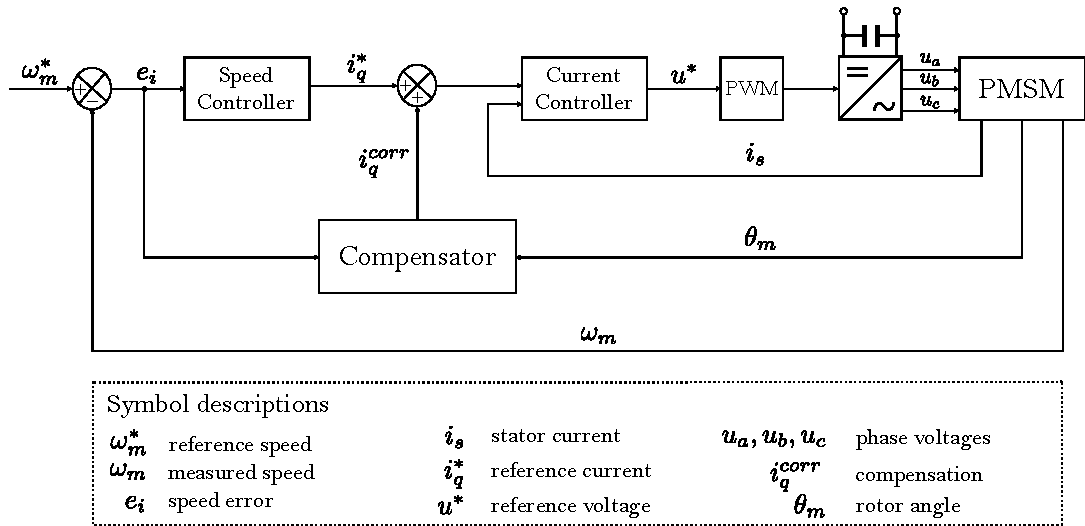
\includegraphics[width=1.0\linewidth]{images/compensator.pdf} 
    \caption{Iterative speed based compensation scheme}
    \label{Compensator_control_diag} 
\end{figure}
%Similarly to RC, ILC can be also combined with an observer, allowing more robust disturbance suppression \cite{ILC:2005, ILC:2018}. Ordinary ILC has two adjustable gains and the compensator can be easily applied to already existing control loop, as can be seen in Fig. \ref{Compensator_control_diag}.

Comparison between RC and ILC is realized in \cite{ILC:RC:R2R:2009}. The conclusion is that the methods could be often considered the same. From now on, ILC will be favoured over RC, because ILC has more strict definition \cite{ILC:1998} and it is recognized more widely \cite{ILC:RC:R2R:2009} as compared to RC. Since angle-based ILC solves the disturbance compensation effectively, the thesis will investigate ILC more carefully in the following chapters.

Neural networks can be iteratively trained to compensate for periodic disturbances \cite{CTR_SW:2017}. The compensation concept is similar to the ILC, but instead of continuously calculating the best compensation value, the network is trained once, thus allowing it to immediately output the best value after training. Implementing a neural network to an old hardware, which must be capable of running real-time processes, can be challenging. Besides limited processing power and memory resources, it can also require a lot of effort to build the network, since modern comprehensive code libraries relying on modern standards, cannot be utilized with old devices.

The training could be done using different hardware than is used in drive. With modern embedded devices capable of connecting to internet, the training could happen on remote servers, which can provide a solution to problems emerging from limited computational resources. However, old embedded devices can rarely connect to internet. Alternative training method could be to use a simulator and then move the trained model to the embedded device by using flash drive for example. However, in such scenario, the model performance is heavily dependant on the simulator accuracy. It can be concluded that neural network based compensation may work with modern products, since such compensators have been already built \cite{CTR_SW:2017}, yet the approach can be troublesome with hardware that does not support modern standards and neither is connected to Internet.

%It is possible to train the network on computer by simulating and then moving the trained model on microcontroller, though such solution can be only as good as the simulator. Dynamic effects such as temperature changes can be hard to model accurately on the simulator. Neural-network based approaches do not currently seem applicable with mass produced drive solutions, although the method appears to be feasible with high-end products that have better machine learning support.

%{\color{blue} Possibly add below that only works reliably with speed control}

\clearpage
